% ------------------------------------------------------------------------------
% SETUP ------------------------------------------------------------------------
% ------------------------------------------------------------------------------

\documentclass[12pt]{article}

\renewcommand{\labelitemi}{$\circ$}
\renewcommand{\labelitemii}{$\circ$}
\renewcommand{\labelitemiii}{$\circ$}

\newcommand{\N}{\mathbb{N}}
\newcommand{\R}{\mathbb{R}}
\newcommand{\setd}{\{1, 2, \dots, D\}}
\newcommand{\setk}{\{1, 2, \dots, K\}}
\newcommand{\setv}{\{1, 2, \dots, V\}}

\usepackage[a4paper, width = 175mm, top = 20mm, bottom = 20mm, 
bindingoffset = 0mm]{geometry}
\usepackage[utf8]{inputenc}
\usepackage[round, comma]{natbib}
\usepackage{url}
\usepackage[font = footnotesize]{caption}
\usepackage{subcaption}
\captionsetup[subfigure]{justification=justified,singlelinecheck=false}
\usepackage{csquotes} \MakeOuterQuote{"}
\usepackage{ragged2e}
\usepackage{array}
\usepackage{tabularx}
\usepackage[fleqn]{amsmath}
\usepackage{bm}
\usepackage{amssymb}
\usepackage{amsthm}
\usepackage{graphicx}
\usepackage{float}
\usepackage[export]{adjustbox}
\usepackage[table]{xcolor}
\usepackage{algorithm}
\usepackage{algorithmic}
\usepackage{xcolor, listings}
\usepackage{textcomp}
\usepackage{fancyhdr}
\newcommand{\changefont}{%
    \fontsize{8}{11}\selectfont
}

\usepackage{refcount}
\usepackage[hang, flushmargin, bottom]{footmisc} 
\usepackage{hyperref}
\hypersetup{
  colorlinks = true,
  linkcolor = .,
  urlcolor = .,
  citecolor = .,
  bookmarks = true}

\newenvironment{tight_enumerate}{
\begin{enumerate}
  \setlength{\itemsep}{0pt}
  \setlength{\parskip}{0pt}
}{\end{enumerate}}

\newenvironment{tight_itemize}{
\begin{itemize}
  \setlength{\itemsep}{0pt}
  \setlength{\parskip}{0pt}
}{\end{itemize}}

\pagestyle{fancy}
\fancyhead{}
\fancyhead[R]{\changefont{Topic-Specific Sentiment Analysis for Tweets by 
German MPs}}
\fancyfoot{}
\fancyfoot[R]{\thepage}
\setlength{\headheight}{14.5pt}
\setlength{\parindent}{0pt}
\interfootnotelinepenalty = 10000

% ------------------------------------------------------------------------------
% MAIN -------------------------------------------------------------------------
% ------------------------------------------------------------------------------

\usepackage{Sweave}
\begin{document}
\Sconcordance{concordance:main.tex:main.Rnw:%
1 80 1 1 0 217 1}


% FRONT PAGE -------------------------------------------------------------------
 
\begin{titlepage}
\begin{center}
    
\LARGE
Statistical Consulting
    
\vspace{0.5cm}
      
\rule{\textwidth}{1.5pt}
\Huge
\textbf{Topic-Specific Sentiment Analysis for Tweets by German MPs}
\rule{\textwidth}{1.5pt}
   
\vspace{0.5cm}
      
\large
Department of Statistics \\
Ludwig-Maximilians-Universität München 

\vfill

\textcolor{red}{Munich, month day\textsuperscript{th}, 2021}
      
\vfill


\includegraphics[width = 0.4\textwidth]{figures/sigillum.png}

\vfill

\begin{tabular}{rl}
  Authors & Asmik Nalmpatian \\
  & Lisa Wimmer \\
  & \\
  Project Partner & Prof. Dr. Paul Thurner \\
  & \textit{Department of Political Science} \\
  & \\
  Supervisors & Matthias Aßenmacher, Ph.D. \\
  & Prof. Dr. Christian Heumann \\
  & \textit{Department of Statistics}
\end{tabular}

\end{center}
\end{titlepage}

% CONTENTS ---------------------------------------------------------------------

\pagenumbering{Roman}
\newpage

\Large
\noindent
\textbf{Abstract}
\vspace{0.5cm} \\
\noindent
\normalsize
\input{chapters/0_abstract.Rnw}
\newpage

\tableofcontents
\newpage

\listoffigures
% \newpage
\vspace{1cm}
\listoftables
\newpage

\Large
\noindent
\textbf{List of Abbreviations}
\vspace{0.5cm} \\
\noindent
\normalsize

\begin{tabular}{rl}
  MP & Member of Parliament \\
  NLP & natural language processing \\
  STM & structural topic model \\
  TSSA & topic-specific sentiment analysis
\end{tabular}

\vspace{1cm}

\Large
\noindent
\textbf{List of Symbols}
\vspace{0.5cm} \\
\noindent
\normalsize

\begin{tabular}{rl}
  $A$ & identity matrix with $s^2$ entries  \\
  $0$ & $s$-dimensional zero vector
\end{tabular}

\newpage

% CHAPTERS ---------------------------------------------------------------------

\pagenumbering{arabic}
    
\section{Introduction}
\label{intro}
\input{chapters/1_introduction.Rnw}

\section{Project Outline}
\label{project}
\input{chapters/2_project.Rnw}

\section{General Theoretical Context}
\label{theory}
\input{chapters/3_theory.Rnw}

\section{Analytical Proposal}
\label{analysis}
\subsection{Data}
\label{data}

% ------------------------------------------------------------------------------

\subsubsection{Data collection}
\label{data_collection}

The subject of our analysis are tweets by members of the German parliament
(\textit{Bundestag}) issued after the last federal election in September 
2017\footnote{
The 2017 Bundestag is comprised of 709 seats and seven political parties: the 
right-wing AfD, the Christian Democrats (CDU/CSU), the Liberals (FDP), the 
Greens, the Left Party, and the Social Democrats (SPD).
CDU/CSU and SPD as ruling parties co-exist in a grand coalition.
}.
Twitter makes these publicly accessible via its official API and the number of 
retrievable tweets per user can be exploited generously, so data supply is 
almost unrestricted.
However, with sentiment classification as ultimate goal of analysis, we face a 
major bottleneck in the need for labeled data.
Lacking the resources for large-scale annotation we did the labeling by hand.
The resulting data set, from a vast amount of available data, consists of 1,215 
observations, imposing some practical limits on the analytical scope.
\\

\textbf{Web scraping.}
For data collection from the Web we rely on the scraping procedure developed in 
the predecessor project, with minor modifications.
The process entails four steps: first, gather MPs' names and basic information 
(such as party affiliation and electoral district) from the official Bundestag 
website; second, find Twitter account names (using individual party websites as 
additional sources); 
third, acquire socioeconomic information for the time of the last 
federal election on a per-district level (available at the official website of 
the federal returning officer); and, lastly, scrape actual tweets along with 
some additional variables like the number of retweets.
We use a \texttt{Python} code base and mainly employ selenium webdrivers as well
as the \texttt{BeatifulSoup} library \citep{richardson2007} for parsing HTML
content and the \texttt{tweepy} library \citep{roesslein2020} for accessing the
official Twitter API.
For more details on the procedure and the large data base assembled in the 
predecessor project please refer to \citet{schulzewiegrebe2020}; the code is 
fully submitted in our electronic appendix and a somewhat more compact demo may 
be found among the teaching material.
\\

\textbf{Data labeling.}
In the data annotation phase we extracted a set with some tens of thousands 
of observations according to the above process and manually selected what we 
deem informative examples.
For these we assigned polarities, i.e., predicates \textit{positive} or
\textit{negative}, and also topic descriptions required for BERT's ABSA task.
We noted in the process that a large number of tweets do not appear to carry 
sentiment at all.
The resulting 1,215 training observations, originated by a total of 256 MPs, 
date from the period of October 2017 to January 2021.
In figure \ref{fig_obs_time} we detect both periodical fluctuations in the 
number of tweets over time and a general upward-sloping trend.

\begin{figure}[H]
  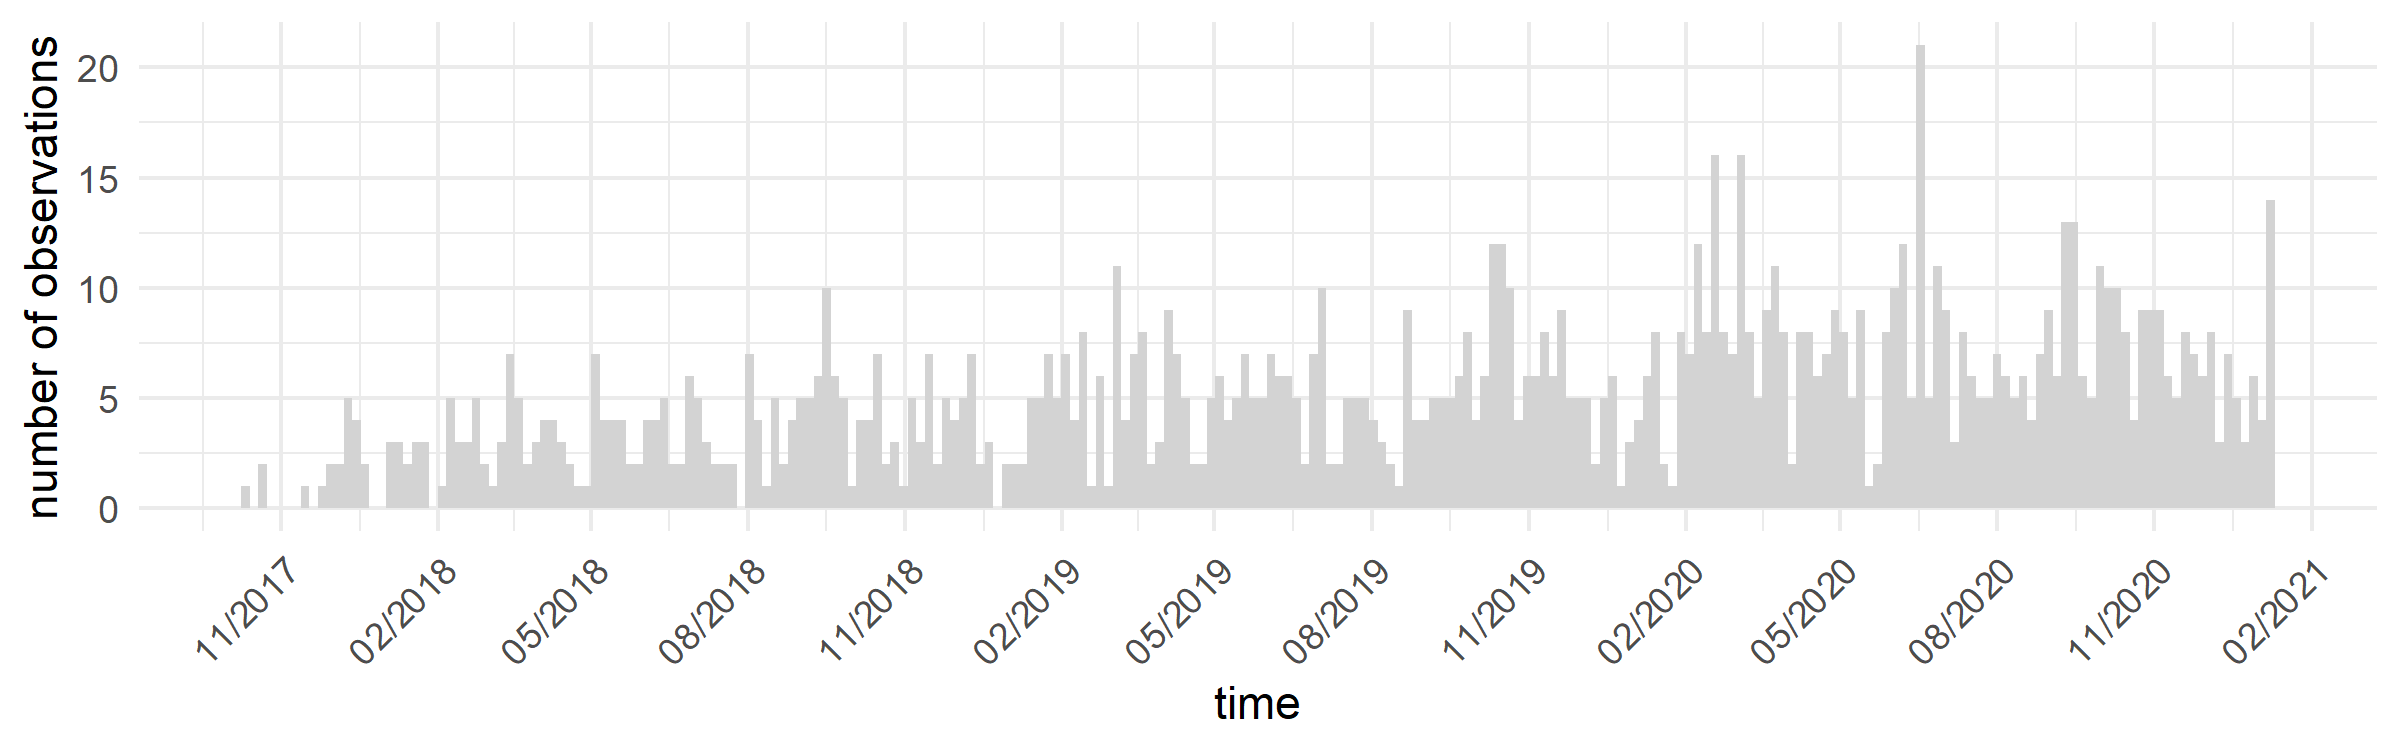
\includegraphics[width = \textwidth]{figures/obs_over_time}
\caption[Training data: observations over time]
{\raggedright Observations over time.}
\label{fig_obs_time}
\end{figure}

An exemplary extract from our training data with some of the most important 
variables is shown in table \ref{tab_extract}.
Exactly which features enter sentiment classification is documented in the 
subsequent chapters.

\begin{table}[H]
  \scriptsize
  \begin{tabular}{l|l|l|l|r|r|l}
  \texttt{username} & \texttt{party} & \texttt{created\_at} & \texttt{text} & 
  \texttt{followers} & \texttt{unemployment\_rate} & \texttt{label}\\
  \hline
  karl\_lauterbach & spd & 2019-12-01 09:44:00 & "Die Wahl ..." & 337001 & 8.5 & 
  negative\\
  \hline
  Martin\_Hess\_AfD & afd & 2018-08-17 07:15:00 & "Vor den ..." & 6574 & 3.5 &
  negative\\
  \hline
  BriHasselmann & gruene & 2019-09-25 15:35:00 & "Ich finde ..." & 20299 & 8.6 
  & positive\\
  \hline
  danielakolbe & spd & 2020-05-12 06:05:00 & "Aber verpflichtend ..." & 8158 & 
  8.3 & negative\\
  \hline
  JuergenBraunAfD & afd & 2020-08-13 22:05:00 & "Panik-Latif + ..." & 3188 & 
  3.4 & negative\\
  \end{tabular}
  \caption[Training data: extract]
  {\raggedright Training data extract for selected variables.}
  \label{tab_extract}
\end{table}

Figure \ref{fig_obs_party} depicts the number of observations per party both 
for our labeled training data and the larger sample from which the training data 
have been selected (containing just over 31,000 tweets).
We notice two things.
First, in either case, the share of tweets (blue) does 
not mirror the share of seats in the Bundestag (gray); most notably, the 
Christian Democrats tweet rather little, whereas the Greens are 
disproportionately active on Twitter.
Second, the right-wing AfD and the Greens are over-represented in our training 
data at the expense of the other groups.
This is simply because these two parties, in our personal experience from the
annotation process, more often issue tweets that are strongly opinionated.

\begin{figure}[H]
  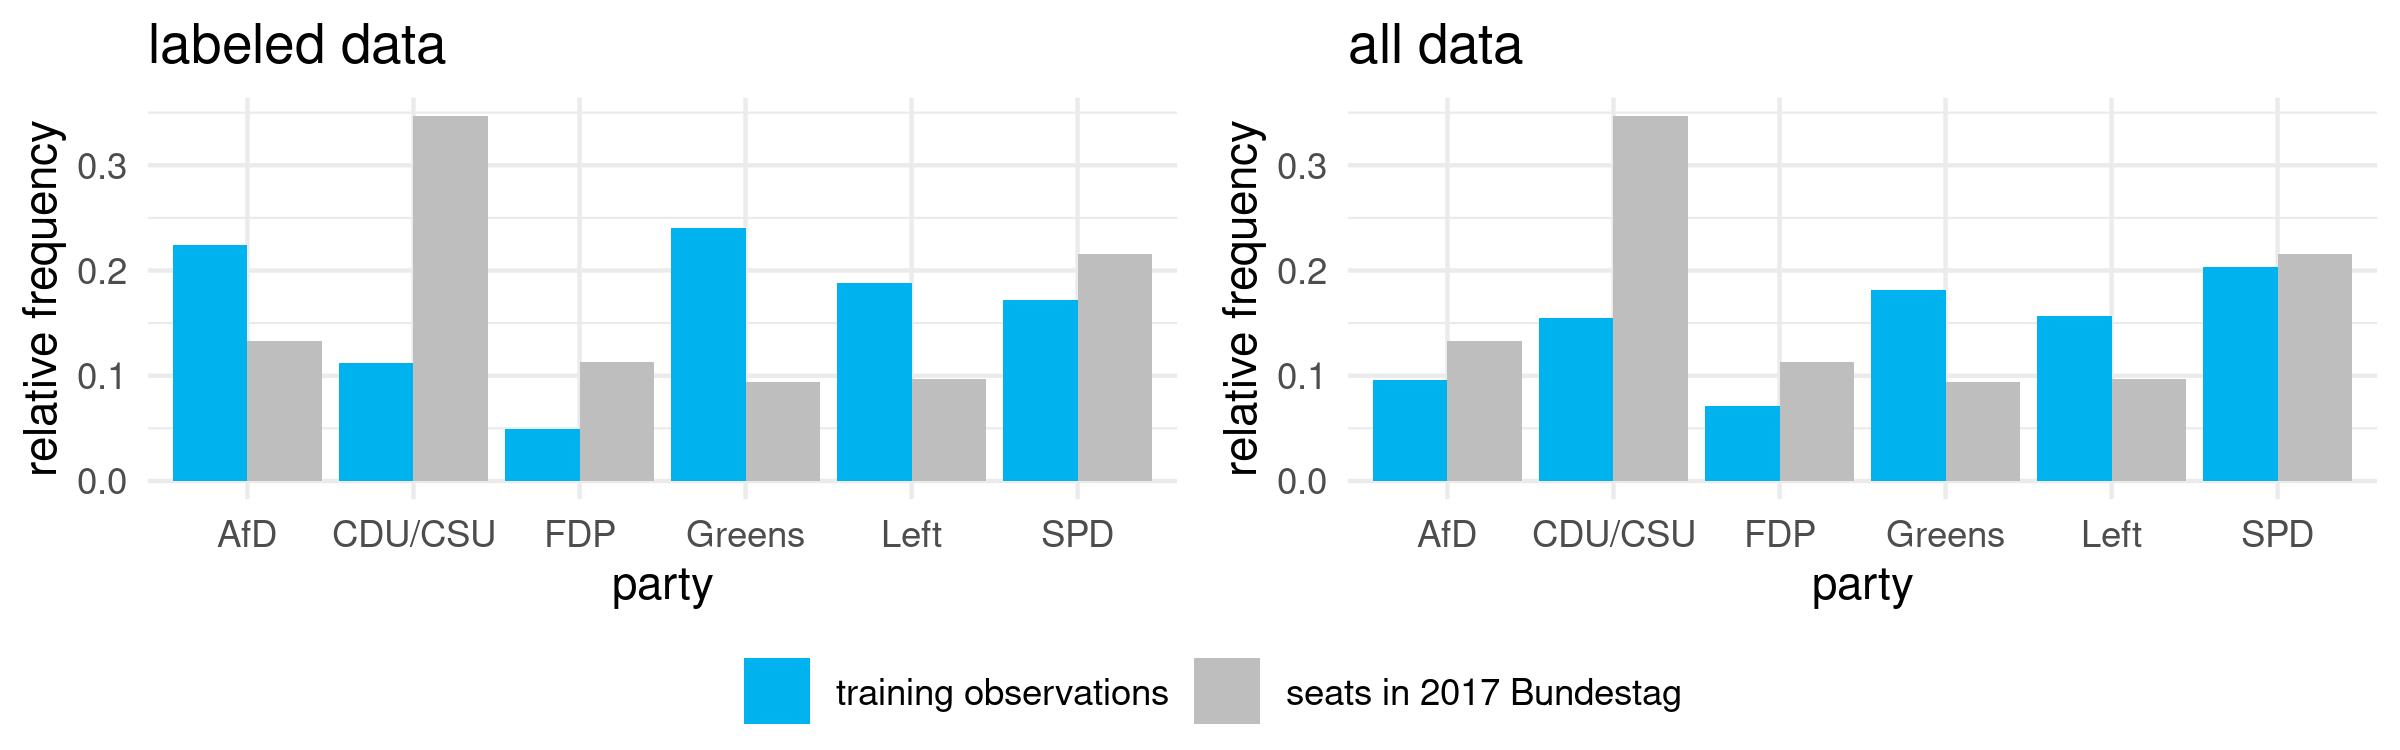
\includegraphics[width = \textwidth]{figures/obs_per_party}
\caption[Training data: observations per party]
{Observations per party in labeled training data (\textit{left}) and entire 
scraped data example (\textit{right}), both depicted against seat distribution 
in current parliament.}
\label{fig_obs_party}
\end{figure}

Lastly, when we inspect the class label distribution in the training data,
an imbalance favoring the negative class becomes immediately visible: some 
72\% of tweets have been marked as negative.
This reflects our general impression that most tweets which do carry sentiment 
express negative opinions and might be partly appropriated to the fact that 
the majority of authors belong to opposition parties.

% \begin{minipage}[b]{0.5\textwidth}
%   Lastly, when we inspect the class label distribution in the training data,
%   an imbalance favoring the negative class becomes immediately visible: some 
%   72\% of tweets have been marked as negative.
%   This reflects our general impression that most tweets which do carry sentiment 
%   express negative opinions and might be partly appropriated to the fact that 
%   the majority of authors belong to opposition parties.
% \end{minipage}%
% \begin{minipage}[b]{0.05\textwidth}
%   \phantom{foo}
% \end{minipage}%
% \begin{minipage}[b]{0.45\textwidth}
%   \begin{figure}[H]
%     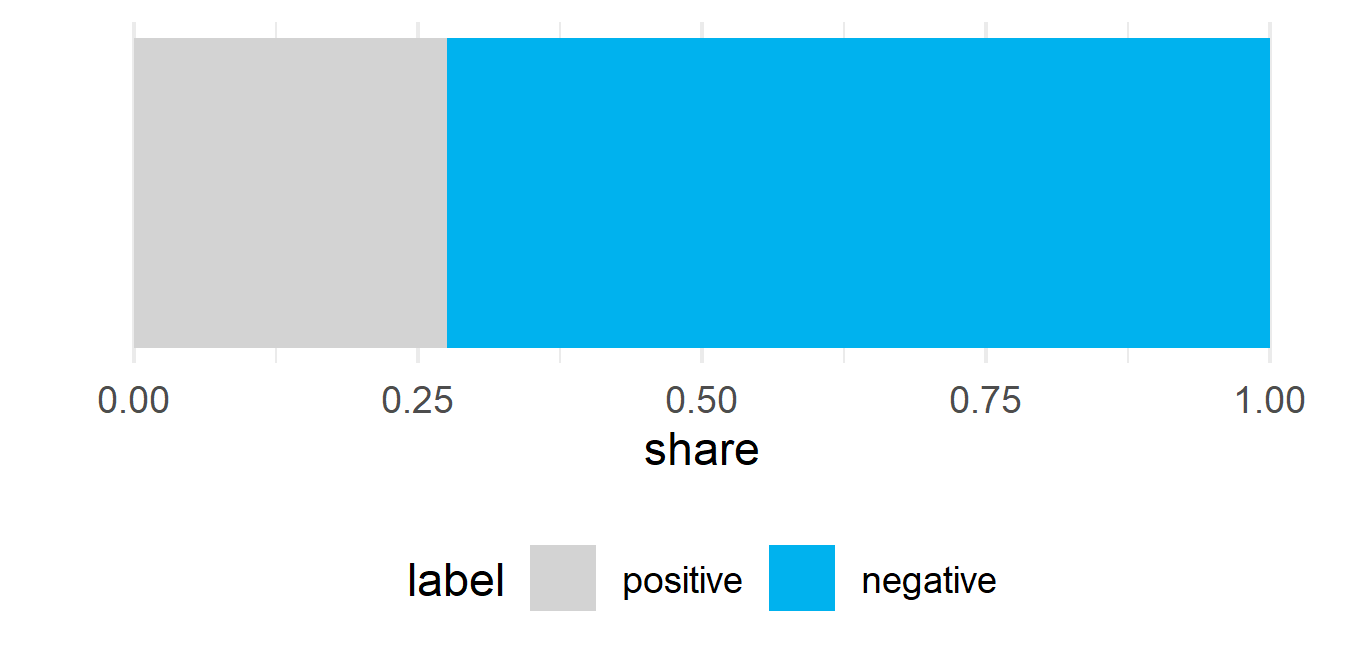
\includegraphics[width = \textwidth]{figures/class_dist}
%     \caption[Training data: class label distribution]
%     {\raggedright Distribution of class labels.}
%     \label{fig_class_dist}
%   \end{figure}
% \end{minipage}%

% ------------------------------------------------------------------------------

\subsubsection{Data pre-processing}
\label{data_preproc}

The standard ML approach requires a lot more feature engineering 
than BERT does, but some general pre-processing steps are applied for both.
In an initial step all tweets in non-German language are excluded from the data.
We proceed with basic text cleaning, namely transcription of 
German umlauts and ligature s into standard-Latin characters and removal of 
non-informative symbols (such as those induced by ampersand conversion). 
The next block of operations is specific to Twitter data and includes the 
identification, separate storage and subsequent removal of special characters 
such as hashtags, emojis and user tags.
By this we ensure the data are available for explicit analysis but do not 
introduce noise in the text.
We finish the pre-processing procedure by assigning a unique identifier to 
each tweet.

% ------------------------------------------------------------------------------

\subsubsection{Challenges}
\label{challenges}

Text data come with many idiosyncrasies to begin with: language is highly 
diverse, irregular, and subject to constant change.
Contextual dependencies and complex constructs such as colloquialisms or sarcasm 
pose serious obstacles in NLP, besides which profanities like spelling or 
translation mistakes must be handled \citep{mohammad2017}.
Some particular properties of the data at hand add to these challenges.
\\

\textbf{Language-specific.}
Not surprisingly, most work in NLP is concerned with the analysis of 
English documents.
Although German is not a low-resource language and attracts its own share of 
research, many analyses and tools are predominantly tailored to English.
German grammar is another aspect that needs to be considered.
Syntax is heterogeneous, and inflections due to cases and genera 
result in many variations of lexical lemmata \citep{rauh2018}.
\\

\textbf{Twitter-specific.}
Tweets' brevity is arguably the most critical issue for analysis.
The limit of 280 characters means that words rarely appear more than once and 
we cannot expect many indicators of topics or sentiments in each document.
It also prompts the use of abbreviations.
On a similar note, we observe that Twitter posts often refer to certain events 
or topical entities without explicitly mentioning them, which is probably both 
due to the character limit and the real-time character of publications.
The message may be clear for an informed human annotator then but will be hard 
to grasp for machines.
Furthermore, tweets tend to be of rather informal style and use language that 
appears almost exclusively in social media, enlarging the vocabulary the 
classifier must understand.
\\

\textbf{Context-specific.}
The context of our data lessens the degree of informality somewhat; the issued 
documents are mostly political statements and as such more akin to written 
texts from other sources.
Still, the political domain introduces new vocabulary yet again and makes the 
transfer of knowledge from other contexts harder.
We also note that sarcasm and irony are frequently applied. 
Lastly, as mentioned before, we find many tweets to be solely informative and 
detect an imbalance toward negative sentiment in those that do convey opinion.

% ------------------------------------------------------------------------------

\subsection{Standard machine learning solution}
\label{tssa_ml}

% ------------------------------------------------------------------------------

\subsubsection{Concept}
\label{tssa_ml_concept}

A number of components make up a typical workflow in supervised ML that adheres 
to the principle of \textit{empirical risk minimization}
(figure \ref{fig_ml_workflow}).

\vspace{0.3cm}

\begin{minipage}[b]{0.45\textwidth}
  Starting from a \textit{task} which consists of (initial) features and one or 
  multiple target values, we train a \textit{learner} on parts of the data.
  The learner encapsulates our beliefs about the feature-target relationship 
  (\textit{hypothesis}) and uses some \textit{optimization} method to produce a 
  model that incurs minimum training loss, or \textit{risk}, according to some 
  metric.
  Applying this usually parameterized model to the observations set aside for 
  testing yields predictions we can compare to the ground truth for 
  \textit{performance evaluation}, again with respect to a given metric. 
  With this, we estimate the true \textit{generalization ability} of our model 
toward unseen data from the same data-generating process.
\end{minipage}%
\begin{minipage}[b]{0.05\textwidth}
  \phantom{foo}
\end{minipage}%
\begin{minipage}[b]{0.5\textwidth}
  \begin{figure}[H]
    \begin{center}
      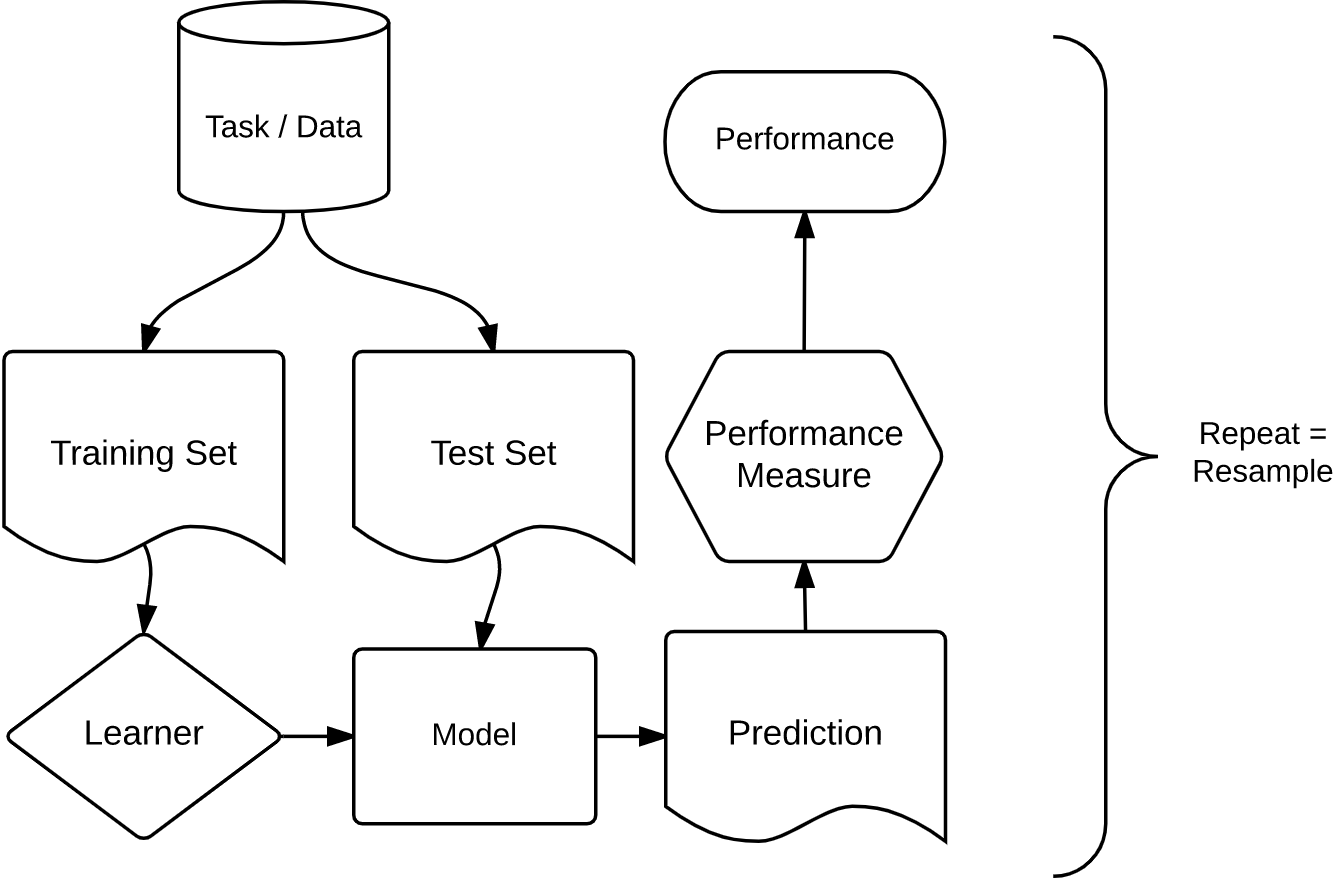
\includegraphics[width = \textwidth]{figures/supervised_learning_schema}
    \end{center}
  \caption[Typical ML workflow]{Typical ML workflow \citep{mlr3book}}
  \label{fig_ml_workflow}
  \end{figure}
\end{minipage}%

\vspace{0.3cm}

As performance might depend rather strongly on the given training data, 
especially if there are few observations to begin with, we will typically 
conduct multiple train-test splits (\textit{resampling}).
Various resampling strategies are available, such as bootstrapping or 
cross-validation.
When the training process requires internal validation steps itself, e.g., for 
hyperparameter tuning, we need a \textit{nested resampling} procedure to ensure 
that no information from training leaks into the test predictions 
\citep{japkowiczshah2011}. 
\\

As figure \ref{fig_ml_workflow} suggests, the workflow is of quite modular 
nature.
We therefore build an automated ML (AutoML) pipeline for sentiment 
classification that allows to repeat training procedures and exchange components 
easily.
Following a pre-training feature extraction phase (referred to as 
\textit{static features}), the pipeline roughly serves 
the purpose of computing topic-specific embeddings (\textit{dynamic features}), 
selecting an appropriate learning algorithm with included tuning step, and 
returning a trained model.
Designing the process this way is beneficial for several reasons:

\begin{enumerate}
  \item \textbf{Dichotomy between train and test sphere.} Topic-specific 
  embeddings are computed globally across several observations.
  In order to actually enable predictions for unseen data, these dynamic 
  calculations must be based solely on the training data.
  Since unbiased learning requires strict separation between train and test
  sphere, we must be careful to wall off predictions at test time from these 
  computations exacted during training.
  The pipeline approach ensures this for each sequence of training and 
  prediction.
  \item \textbf{Automatization.} Automating (parts of) algorithm selection and 
  hyperparameter tuning helps with crucial design decisions by attaching them to 
  the given data.
  \item \textbf{Transferability.} The possibility to plug in alternative 
  components makes the 
  approach instructive also for different applications.
\end{enumerate}

In the following, we explain in more detail the two different stages of feature 
extraction, introduce the learners we propose to include, and show how the 
final pipeline is assembled.

% ------------------------------------------------------------------------------

\subsubsection{Feature extraction}
\label{tssa_ml_feat}

\textit{\textbf{Static features}}
\\

Static feature extraction forms the first block of the standard ML procedure and 
provides tabular data which then enter the AutoML pipeline.
We refer to these features as static because they can be calculated prior to any 
training process, depending solely on single observations.
They are based on the so-called \textit{bag-of-words 
(BOW)} assumption that leads to texts being treated as arbitrary collections of 
vocabulary instances.
In particular, information about grammar and word order is discarded in BOW 
approaches.
This is obviously a strong simplification but hard to avoid entirely with 
standard classifiers \citep{cambriaetal2017}.

The static feature extraction steps rely heavily on \texttt{R}'s 
\texttt{quanteda} package \citep{pkgquanteda} for organizing documents in corpus 
objects, tokenizing texts and performing look-ups with dictionaries.
We use lists of stopwords in multiple places to exclude uninformative 
tokens such as determiners or auxiliary verbs.
These are compilations from various sources, including \texttt{quanteda}'s 
built-in list, open-source data available on 
\href{https://github.com/stopwords-iso/stopwords-de}{GitHub} and some manually 
appended, domain-specific terms. 
In addition, we repeatedly apply \textit{stemming} in order to reduce words to 
their root form (for instance, cutting back both \textit{"works"} and 
\textit{"working"} to \textit{"work"}).

All of these operations are aimed at compressing document representation from 
the total of unique original terms to more generalized tokens that co-occur 
across texts
This way we create features that are actually shared by multiple observations 
and thus help classifiers infer feature-target relations with the ability to 
generalize.
For the static part we exploit insights from other studies 
(e.g., \citet{balyetal2017}, \citet{correaetal2017}, \citet{jabreelmoreno2017}, 
\citet{sidarenka2019})
and include the following features: 

\begin{enumerate}

  \item \textbf{Lexicon-based polarity counts.} These comprise two sources of 
  prior polarity, namely words and emojis. 
  We use the aggregate of three large German polarity-term dictionaries, 
  \textit{GlobalPolarityClues} \citep{waltinger2010}, \textit{SentiWS} 
  made available \href{https://wortschatz.uni-leipzig.de/en/download}{online}
  by Leipzig university and a collection by \citet{rauh2018}, for word 
  polarities.
  The resulting lexicon distinguishes weak and strong sentiment.
  In each tweet, if a word is part of the dictionary and judged to have 
  either positive or negative connotation (weak or strong), it raises the 
  respective polarity count by one.
  Emojis are treated analogously, albeit without the discrimination between 
  degrees of sentiment, using an emoji polarity list accumulated by 
  \citet{kraljetal2015}.
  
  \item \textbf{Twitter variables.} We make use of the additional information 
  provided by the Twitter API and note for each tweet the number of likes and 
  retweets as well as the number of users tagged.
  For hashtags we resort to the same naive measure since we find them to be so 
  heterogeneous across documents in our training set that no meaningful 
  information can be extracted. 
  This certainly marks an opportunity for future improvement.
  
  \item \textbf{Syntactic features.} This group attempts to mitigate the 
  simplification introduced by the BOW assumption to some extent.
  We track the presence of modifiers that indicate sentiment intensification 
  as well as punctuation via the respective number of quotation and exclamation 
  mark.
  Negation is a delicate problem we currently treat with the brute-force 
  approach of noting whether or not negating tokens are present.
  German language complicates negation handling by the fact that modifier and 
  modification target often appear in quite separate sentence positions, making 
  it hard to identify the actually negated construct in an automated manner.
  
  \item \textbf{Character unigrams.} Unigrams refer to single tokens (whereas 
  $n$-grams mean the concatenation of $n$ tokens) and we consider the special 
  case of character tokens, meaning we count the occurrence of single letters.
  While this may not seem too helpful at first glance, character unigrams 
  lead to a very dense document representation as opposed to the sparsity 
  induced by word unigrams or even bi- and trigrams.
  
  \item \textbf{Part-of-speech (POS) tags.} The last type of features captures 
  grammatical structure.
  POS tags are used to categorize sentence parts according to their syntactic 
  role.
  Including these stems from the idea that the number of certain tags, for 
  example adjectives and adverbs, might indicate sentiment.
  % We use the \texttt{spacyR} package \citep{pkgspacyr}, a wrapper around 
  % \texttt{Python}'s \texttt{spaCy} library closely integrated with 
  % \texttt{quanteda}, for POS tagging.
  
\end{enumerate}

\vspace{0.3cm}

\textit{\textbf{Dynamic features}}
\\

The static features are not in any sense topic-specific.
In order to allow for sentiments to vary across topics, we include 
topic-specific word embeddings.
This entails a two-step procedure: first, we group documents with an STM, 
and then compute word embeddings for each topical cluster. 
\\

\textbf{Topic modeling.}
The STM \citep{robertsetal2016} is a generative topic model and attempts to 
recreate the very process that generated the observed documents.
As sketched in section \ref{tm}, this is achieved by sampling topic proportions 
for each document from some distribution, assigning word positions to topics 
with the resulting probabilities, and drawing vocabulary instances from the 
distribution associated with the respective topic.
As opposed to the original LDA approach assuming a single global prior 
distribution, the STM offers the possibility to incorporate document-level meta 
data. 
These may affect the sampling process in two places: first, by influencing the 
topic proportions for a given document (\textit{topical prevalence}), and 
second, by altering the distribution the vocabulary assumes over each topic 
(\textit{topical content}).
Our case lends itself more to using topical prevalence variables, presuming that 
certain meta features on electoral district level, which can be specified in 
terms of an additive formula, have an impact on which topics are discussed.
Defining a topical content variable (a single, categorical one is supported in 
the STM implementation \citep{pkgstm}) allows for topic-word distributions to 
vary for its different levels.
Such an approach is also conceivable but not further pursued here.
The STM can be expressed by the following generative process\footnote{
We adopt the notation from \citet{schulzewiegrebe2020} for consistency.
} for each document $d \in \setd$ \citep{robertsetal2016}:

\begin{enumerate}

  \item Draw non-normalized topic proportions $\bm{\eta_d}$ from a 
  $(K - 1)$-dimensional Gaussian: 
  $\bm{\eta_d} \sim \mathcal{N}_{K - 1}(\bm{\Gamma}^T\bm{x}_d^T, \bm{\Sigma})$, 
  where the $K$-th component is set to zero to keep the model identifiable.
  $\bm{x}_d$ is the vector of $P \in \N$ prevalence covariates associated with 
  document $d$, and $\bm{\Gamma} \in \R^{P \times K}$ is a matrix of topic 
  proportion coefficients obtained by means of Bayesian linear regression with 
  Gaussian priors and first-order penalty term.
  The covariance matrix $\bm{\Sigma}$ can have arbitrary structure and thus 
  incorporate inter-topic correlations.
  
  \item Normalize $\bm{\eta_d}$ through a softmax operation, 
  yielding $\bm{\theta}_d$ with $\theta_{d, k} = \frac{\exp(\eta_{d, k})}{
  \sum_{j = 1}^K \exp(\eta_{d, j})}$, $k \in \setk$. 
  The $\bm{\theta}_d$ then effectively follow a logistic normal distribution. 
  
  \item For each word position $n \in \{ 1, 2, \dots, N_d \}$:
  
  \begin{enumerate}
    \item Draw $\bm{z}_{d, n} \sim \mathit{Multinomial}(\bm{\theta}_d)$ to 
    assign the $n$-th position to a topic. 
    \item Draw a word $w_{d, n}$ from the word distribution corresponding to the 
    assigned topic: $w_{d, n} \sim \mathit{Multinomial}(\bm{\beta}(d, n))$.
  \end{enumerate}
  
\end{enumerate}

For our analysis we include a total of four prevalence covariates, namely the
MP's party affiliation and federal district (\textit{Bundesland}) as well as 
the share of migrant population and overall employment rate.
The latter two are modeled as smooth effects with five degrees of freedom each.
While we find this formula to work well with our particular training data, the 
specification can be easily modified.
\\

\textbf{Word embeddings.}
We now use the information from topic assignment to compute topic-specific word 
embeddings.
Recall that the BOW assumption results in very high-dimensional document 
representations disregarding inter-term relationships.
Word embeddings seek to capture semantic structures in these representations: 
words are characterized by their surrounding context and projected into a latent 
space in which similar words end up in nearby locations.
At the same time, embeddings perform dimensionality reduction as the latent 
space is typically chosen to be of much lower dimension than the 
observation space.

We use the\textit{Global Vectors (GloVe)} model proposed by 
\citet{penningtonetal2014} and implemented in \texttt{R} by \citet{pkgtext2vec}.
Its computation is based on the symmetric \textit{co-occurrence matrix} 
$C \in \R^{M \times M}$, where $M \in \N$ denotes the number of tokens remaining 
after such pre-processing steps as stopwords removal.
Entry $c_{i, j}$ states how often token $j$ occurs in the context of token $i$.
Context is a local notion controlled via \textit{window size} $\ell \in \N$, 
where $\ell$ specifies the number of positions to each side of a token
considered to be in its vicinity, the underlying (simplifying) assumption being 
that the strength of semantic relation decays with increasing distance.
The entries of the co-occurrence matrix are weighted by the inverse 
distance to the target token.
We can therefore express probabilities of co-occurrence as fractions of row (or 
column) sums: the probability of the $i$-th word occurring in the context of 
the $j$-th word is given by $p_{ij} = \tfrac{c_{ij}}{c_{i.}}$ with $c_{i.}$ 
as the $i$-th row sum.
The co-occurrence probabilities in turn give rise to odds 
$\frac{p_{ik}}{p_{jk}}$, for which \citet{penningtonetal2014} posit that they 
should be reflected by embedding vector distances.
This is formalized as 

\begin{equation*}
  \exp((q_i - q_j)^T \tilde q_k) = \exp(q_i^T \tilde q_k - q_j^T \tilde q_k) = 
  \frac{p_{ik}}{p_{jk}},
\end{equation*}

with $q_i \in \R^m$, $m \in \N$, as the $m$-dimensional embedding vector 
representation for word $i$.
$\tilde q_k$ is structurally equivalent to $q_k$ for symmetric $C$ and 
differences arise solely from different random initialization of the model.
The authors do not provide a sound theoretical foundation for this double 
computation but point out that such stochastic variance has been shown to 
benefit overparameterized models.
In the end GloVe actually uses the sum of the vectors as embeddings.
We arrive at $q_i^T \tilde q_j + b_i + \tilde b_j \approx \log(c_{ij})$,
with bias $b_i$ approximately equal to $\log(c_i)$, and can now express the 
embedding error minimization problem with the following weighted least-squares
objective::

\begin{equation*}
  \min_{\bm{v}, \bm{b}} \sum_{i = 1}^M \sum_{j = 1}^M g(c_{ij}) \left(
  q_i^T \tilde q_j + b_i + \tilde b_j - \log(c_{ij}) \right)^2.
\end{equation*}

$g$ is a weighting function for which the authors propose to use

\begin{equation*}
  g(x) = \begin{cases} \left( \frac{c_{ij}}{c_{\mathit{max}}} \right)^{\alpha} & 
  c_{ij} < c_{\mathit{max}}, \\
  1 & \text{otherwise}.
  \end{cases}
\end{equation*}

$c_{\mathit{max}}$ and $\alpha$ are hyperparameters to the GloVe algorithm, as 
are the embedding dimensionality $m$ and the size of the context window $\ell$ 
\citep{penningtonetal2014}.
\\

GloVe returns an embedding vector for each word.
Since we are interested in a representation on document level, the word 
embeddings are aggregated in a final step.
This leaves us with a block-like structure of embedding vectors: for $K$ topics 
and $m$ embedding dimensions we obtain $K \cdot m$ features vectors, where each 
document has non-zero entries only for the columns corresponding to its 
associated topic.
At the end of the entire feature-generating process we can thus describe our 
documents by a number of static covariates plus topic-specific embedding values.
This tabular representation of our Twitter corpus forms our classification task.

% ------------------------------------------------------------------------------

\subsubsection{Sentiment classification}
\label{classifiers}

We propose two different classification algorithms, a \textit{random forest} and 
a logistic regression learner with elastic net penalty (\textit{glmnet}).
Both ship with built-in feature selection, which we consider rather helpful in 
the potentially high-dimensional feature space of text classification, and are 
fairly easy to tune (\citet{japkowiczshah2011}, \citet{probstetal2019}).
However, the pipeline design allows to plug in any other suitable learner 
instead.
\\

\textbf{Random forests.}
A random forest is an ensemble of tree base learners \citep{louppe2014}.
Starting from a root node containing all observations, classification trees 
perform subsequent binary splits of the feature space, repeatedly dividing it 
into rectangular partitions along one dimension at a time.
Observations are passed along the resulting decision tree and end up in a 
particular end node, or leaf, where they are assigned the most frequent 
class label in this node.
In the end, this constitutes hypotheses of the form 
$f(\bm{x}) = \sum_{t = 1}^T c_t \mathbb{I}[\bm{x} \in Q_t]$, where $T$ denotes 
the number of terminal regions $Q_1, Q_2, \dots, Q_T$ and 
$c_t \in \{0, 1\}$ is the class label predicted for observations in leaf node 
$Q_t$.
Each split is constructed such that the empirical risk across all child nodes 
is minimized, which typically corresponds to minimizing class impurity.
To this end, trees perform a greedy search that requires assessing all 
possible splitting variables and associated thresholds
\citep{breimanetal1984}.

Without regularization, i.e., constraining tree depth, classification trees 
will perfectly fit the patterns they observe and may thus change strongly with 
small alterations of the training data.
Random forests exploit the low bias of trees and assemble $B \in \N$ of them to 
reduce variability.
Predictions are obtained by aggregating predicted class labels of all base 
learners (typically, a majority vote is used).
Randomness enters in two ways: first, the subset of data used to fit a single 
tree within the ensemble is chosen at random via bootstrapping, and second, each 
base learner is allowed to use only a random subset of features as splitting 
criteria.
This procedure enables decorrelation and enhances ensemble stability 
\citep{louppe2014}.

Tunable hyperparameters of random forests include ensemble size, the number of 
candidate features to be considered at each split, and various attributes 
associated with single trees' complexity \citep{probstetal2019}.

Random forests easily handle all types of features, including arbitrary 
interactions, and perform natural variable selection.
They mitigate much of single trees' instability and still achieve good 
performance in many applications \citep{louppe2014}.
\\

\textbf{Regularized logistic regression.}
Logistic regression is a special case of generalized linear regression where 
the predictor is linear in the parameters but transformed by a 
possibly non-linear link function \citep{lindsey1997}.

Consider the feature matrix $\bm{X} = [\bm{x}_d^T]_{d = 1, 2, \dots, D} 
\in \mathcal{X} \subset \R^{d \times p}$ and let $\bm{y} \in \{0, 1\}^D$ denote 
the binary sentiment target.
Logistic regression models the probability of $y_d = 1$ for a 
given observation $\bm{x}_d$ as $\pi(\bm{x}_d) = \mathbb{P}(y_d = 1 ~ \rvert +
\bm{x}_d) = \tfrac{\exp(\theta_0 + \bm{\theta}^T\bm{x}_d)}{1 + \exp(\theta_0 +
\bm{\theta}^T\bm{x}_d)}$, with regression coefficients $(\theta_0, \bm{\theta}) 
\in \R^{p + 1}$ \citep{lindsey1997}.
Prediction of class labels requires thresholding the posterior probabilities.
By application of the logit transformation we obtain the linear 
predictor $\theta_0 + \bm{\theta}^T\bm{x}_d = \log 
\tfrac{\pi(\bm{x}_d)}{1 - \pi(\bm{x}_d)}$.

Here, $(\theta_0, \bm{\theta})$ is estimated by minimizing a penalized version 
of the negative log-likelihood.
The additive elastic net penalty balances absolute and quadratic regularization,
in a hybrid of LASSO and Ridge regression. 
Regularization causes shrinkage in the coefficients (typically not affecting the 
intercept) and leads to the following optimization problem , where 
$\lambda \in \R$ and $\alpha \in [0, 1]$ are hyperparameters that need to be 
tuned \citep{hastieetal2021}:

\begin{equation}
    \min_{(\theta_0, \bm{\theta}) \in \R^{p + 1}} - \frac{1}{n} \sum_{d = 1}^D
    y_d (\theta_0 + \bm{\theta}^T\bm{x}_d) - \log(1 + 
    \exp(\theta_0 + \bm{\theta}^T\bm{x}_d)) +
    \lambda \left( (1 - \alpha) \| \bm{\theta} \|_2^2 \cdot \tfrac{1}{2} + 
    \alpha \| \bm{\theta} \|_1 \right ).
    \label{eq_glmnet}
\end{equation}

% ------------------------------------------------------------------------------

\subsubsection{Automated machine learning pipeline}
\label{pipeline}

We assemble all components presented above in an AutoML pipeline.
The pipeline takes care of

\begin{tight_enumerate}
  \item computing the dynamic features, i.e., topic-specific embeddings,
  \item selecting and training the best learner, including hyperparameter 
  optimization, and
  \item predicting sentiment labels for new observations.
\end{tight_enumerate}

We implement the algorithm as a graph learner in the \texttt{mrl3} ecosystem
\citep{pkgmlr3}.
Graph learners are composed of nodes that perform operations on the data.
Multiple options for creating and re-uniting branches enable arbitrarily 
complex constructions.
The design allows to use the entire pipeline just like any other learner object 
in standard ML procedures such as training, prediction, tuning or benchmarking.
\texttt{mrl3}'s internal structure ensures the dichotomy between train and test 
sphere in every step and makes our implementation compatible with other
routines.
\\

\textbf{Pipeline components.}
The proposed pipeline takes a static feature representation of our annotated 
training data and starts by assigning topic labels, afterwards computing 
topic-specific embeddings.
The next block conducts the entire tuning process, where the 
selection of a learner is directly included, such that the optimal classifier is 
found in joint optimization of algorithm and associated hyperparameters.
We rely on existing functionalities for much of the required steps.
However, we contribute custom implementations for the STM and the subsequent 
embedding computation with GloVe.
Embeddings can also be calculated without a preceding topic modeling step.
Furthermore, an alternative topic modeling approach is available. 
It is a non-stochastic procedure that accepts manually defined keywords and 
finds all documents associated with the terms or derivatives thereof.
If necessary, this can be combined with a stratification step that approximately 
retains the ratio of documents associated with a keyword in each resampling 
step.
All these novel operations are constructed as so-called \textit{pipe operators}
in \texttt{mlr3}.
Eventually, the pipeline assumes the following structure: \textcolor{red}{FIG}.
\\

\textbf{Settings.}
Our design choices are partly inspired by \citet{probstetal2019} and otherwise 
reflect what we find to work best.
The decision to compute topic-specific embeddings and the selection 
of learners is such a choice already.
We further fix some hyperparameters in advance to reduce computation time. 
This includes capping the maximum number of iterations in regularized 
regression at 1000 and limiting tree growth in the random forest (leaf nodes 
must contain at least 5\% of observations) as well as allowing for parallel 
computations. 
Other hyperparameters, by contrast, are left to tuning.
The first two are the number of topics with $3\leq K \leq 6$ and the 
dimensionality of embeddings $10\leq m \leq 50$, 
where we exploit the fact these inherently unsupervised problems are input to a 
supervised learning task. 
We can therefore simply have the algorithm choose the configuration that yields
the best predictive performance.
For the actual classification part we allow optimization of the penalty 
coefficients in logistic regression ($0 \leq \alpha \leq 1$ and $0 \leq \lambda
\leq 0.2$) and the number of candidate features for split computation in the 
random forest (limited to 50\% of features at most), as well as the fraction of 
observations to be sampled for each base learner (between 0.25 and 1).
Note that the search space remains rather small; more tuning parameters, larger 
ranges and/or more configurations can be explored with enough computational 
resources.

We use three-fold cross validation (3-CV) as resampling strategy in both the 
outer (performance evaluation) and inner (hyperparameter tuning) training loop.
3-CV divides the training data into three roughly equal-sized partitions, each 
of which serves as test set once while the other two form the training data 
\citep{japkowiczshah2011}.
Tuning is conducted via random search with a total budget of 50 evaluations 
(again, this should be extended if affordable).
Random search is based on the simple idea of drawing from the space of possible 
configurations uniformly at random.
While implementation is easy and readily parallelizable, the number of 
evaluations required to sample the space adequately rises exponentially with the
number of dimensions, with no possibility to learn from prior draws 
\citep{feurerhutter2019}.
Lastly, in the inner tuning loop, we evaluate performance by means of accuracy 
(i.e., the share of correctly classified instances), as we identify no need to 
emphasize one side of misclassification or the other in any particular way.

% ------------------------------------------------------------------------------

\subsubsection{Results}
\label{tssa_ml_results}

% ------------------------------------------------------------------------------

\subsection{Deep learning solution}
\label{tssa_dl}

% ------------------------------------------------------------------------------

\subsubsection{Deep transfer learning with BERT}
\label{bert}

\color{red}

The second part of our work is based on the Bidirectional Encoder 
Representations from Transformers (BERT) and its variations. The name comes from its core architecture as a multi-layer bidirectional Transformer encoder. 
% (https://arxiv.org/pdf/1810.04805.pdf)
The Transformer-based models especially in the recent NLP research consist of 
transfer learning and attention. In standard supervised learning approach, where 
we ideally have a large number of labelled training instances, we assume the 
test data to be drawn from the same distribution in order to test the goodness 
of generalization in a reliable way. Yet, given another domain, for example 
another set of documents with different thematic context, we cannot expect our 
model to generalize well. 
In many situations, as well as in our data situation, one has to (manually) 
label a large amount of data instances, which is not practicable at all. So, 
in data situations where the number of annotated training documents is 
restricted, it becomes hard to deal with the highly resource intensive 
supervised learning. Therefore, it is appropriate to apply the transfer learning 
that represents the approach of statistical learning in which we firstly train 
a model on an original task and domain and then transfer this learned knowledge 
to the target task and domain. The detailed workflow of Transformer is described 
in a paper by researchers at Google AI Language. 
(Pan, S. J. and Yang, Q. (2010). A survey on transfer learning. 
IEEE Transactions on Knowledge and Data Engineering, 
% https://ieeexplore.ieee.org/document/5288526 )

(Ruder, S. (2019). Neural transfer learning for natural language
processing. PhD thesis, National University of Ireland.
% https://ruder.io/thesis/neural transfer learning for nlp.pdf.)
Moreover, the Transformer based architectures do not process the sequential data 
(such as texts) in order, by utilizing the mechanism of attention. Due to this 
property, these architectures allow for much more parallelization than a 
standard RNN and leads to reduced training times. 
% (https://arxiv.org/pdf/1706.03762.pdf)
This is mainly achieved in the pretraining task of a BERT model on a large 
corpus in a specific language with the help of neural networks. In the 
fine-tuning step, this knowledge (so the parameter values learned during 
training the source model) is then applied to a new purpose-specific context to 
learn a certain task and vocabulary. (Devlin, 2019)

% ------------------------------------------------------------------------------

\subsubsection{Input pre-processing}
\label{bert_preproc}

% Die Ausgrenzung von MigrantInnen von der #EssenerTafel ist inakzeptabel und 
% rassistisch. Wir dürfen nicht zulassen, dass die Ärmsten gegeneinander 
% ausgespielt werden.

In order to apply BERT, one has to process the textual input to the encoder of 
BERT. For that, we split the words into tokens or wordpieces based on a given 
vocabulary, which is determined by the pretrained language model. Then convert 
each sequence of tokens into numerical vectors, embeddings and process them in 
the neural network with some additional tokens: The beginning of the first 
sequence is signed by a “[CLS]” token, the end by a “[SEP]” token. Due to a 
marker Sentence A or B to each token in a sequence helps to indicate which 
sentence a token belongs in. Moreover, a positional embedding stands for the 
position of each token in the sentence. The inputs have to be of same length, 
whereby the maximum length of an input sequence can be 512 tokens. Shorter 
inputs are filled with padding tokens and the longer ones are truncated.

% [CLS] Die Ausgrenzung von MigrantInnen von der # EssenerTafel ist inakzeptabel 
% und rassistisch. Wir dürfen nicht zulassen, dass die Ärmsten gegeneinander 
% ausgespielt werden. [SEP]

% ------------------------------------------------------------------------------

\subsubsection{Pre-training}
\label{bert_pretrain}

Originally, BERT was pretrained on a huge corpus of Wikipedia texts. In order 
to cope with the challenges of a directional approach while predicting the next 
word in a sequence, BERT uses two basic strategies during pretraining: Masked 
Language Modelling and Next Sentence Prediction.
\\

\textbf{Masked language modeling (MLM).}
By masking a random word, BERT tries to predict this independent from its 
positioning in the sequence. As BERT is able to work in bidirectional way, that 
is to condition the predictions for the masked word on the co-occurred words on 
both sides, it is able to capture different and more flexible information about 
the context of a certain word. After randomly choosing  15\% of the token 
embeddings, the 80\% of them will be replaced by the “[MASK]” token, in 10\% of 
the cases, the masked tokens are replaced by a random token (different) and in 
the 10\% remaining cases, the masked tokens are left unchanged. Afterwards these 
sequences are fed into the BERT model. (Devlin, J., Chang, M.-W., Lee, K., and 
Toutanova, K. (2019). BERT: Pre-training of deep bidirectional Transformers for 
language understanding.)
% [CLS] Die Ausgrenzung von [MASK] von der # EssenerTafel ist inakzeptabel und 
% [MASK]. Wir dürfen nicht zulassen, dass die [MASK] gegeneinander ausgespielt 
% werden. [SEP]
\\

\textbf{Next sentence prediction (NSP).}
Furthermore, to capture the relationship between two sentences BERT learns to 
predict whether the second sentence in a pair is the follow-up one in the 
original document or not. In the training procedure the half of the inputs are 
originally a pair, while the other half consists of a random sentence from the 
corpus as second sentence. The goal is to make BERT distinguish between real and 
fake pairs. 
These both strategies are applied together in order to minimize the additively 
combined loss function.

% Input: 
% Sentence A: [CLS] Die Ausgrenzung von [MASK] von der # EssenerTafel ist 
% inakzeptabel und [MASK]. [SEP]
% Sentence B: Wir dürfen nicht zulassen, dass die [MASK] gegeneinander ausgespielt 
% werden. [SEP]
% Label: IsNextSentence
% 
% Sentence A: [CLS] Die Ausgrenzung von [MASK] von der # EssenerTafel ist 
% inakzeptabel und [MASK]. 
% Sentence B: [SEP] Freue mich sehr für ihn und auf die Zusammenarbeit. [SEP]
% Label: NotNextSentence

% ------------------------------------------------------------------------------

\subsubsection{Fine-tuning}
\label{bert_fine}

BERT can be used for various language tasks, for example Question Answering, 
Named Entity Recognition, Sequence Classification, etc. The latter one was used 
in this project. To train the pretrained network on a certain task, we need to 
fine-tune BERT on the target task and use the available (limited) labelled data. 
This means, we only have to exchange the output layer adapted for the target 
task. In our case, we used the huggingface pytorch implementation 
BertForSequenceClassification 
% (https://huggingface.co/transformers/model_doc/bert.html#tfbertforsequenceclassification)
, which adds a single linear layer on top for classification.  During the 
fine-tuning all BERT parameters are updated. (Devlin 2018) We set the following 
parameters recommended to use for fine-tuning by the authors: a minibatch size 
of 16 sequences, a global Adam learning rate of 2e-5 and 4 as number of epochs. 
(Devlin 2019)

% ------------------------------------------------------------------------------

\subsubsection{Aspect-based sentiment analysis}
\label{bert_absa}

The Aspect Based Sentiment Analysis is a more sophisticated approach than a 
standard text-level sentiment analysis. Apart from classifying a given text, in 
this case a tweet, it focuses on extracting aspects mentioned in a given text 
and base the classification result on it, together with the tokens contained in 
the text in hope to extract the most relevant information from the textual data. 
For our data situation, the most appropriate approach is therefore the 
methodology described by Hu Xu 
% (https://www.aclweb.org/anthology/N19-1242.pdf)

\textbf{Post-training.}
The basic pretrained BERT model used in our work is the “bert-base-german-cased” 
model, as we deal with tweets in German language and expecting to have 
advantaged with the chance that letter casing will be helpful, because all nouns 
start with the capital letter in German. This model was originally pretrained 
using the latest German Wikipedia texts, news articles and Open Legal Datasets 
of German court decisions and citations. The dataset has a size of ca. 12 GB in 
total. 
% (https://deepset.ai/german-bert)
%  (http://openlegaldata.io/research/2019/02/19/court-decision-dataset.html)
In order to improve both the domain and task knowledge the authors recommend to 
apply a so-called posttraining task based on contextually related data because 
fine-tuning BERT directly with a limited amount of labelled data may end up with 
domain and task challenges. The posttraining on domain knowledge is applied by 
using the pretrained weights as initialization and leveraging the both 
pretraining tasks MLM and NLP. The weights will be updated based on the sum of 
the losses of both tasks. 
\\

\textbf{Aspect extraction.}
The Aspect Extraction task is supposed to find aspects in a given text that the 
reviewer or in our case the user of the twitter account has commented on. The 
idea is to use a supervised technique and label each token from a sequence with 
one of these three labels: “B” – Beginning of an aspect, “I” – Inside of an 
aspect term and “O” – Outside of an aspect. Afterwards for each position of the 
sequence a dense layer and a softmax is applied to predict one of the three 
labels for all positions of a sequence. As shown in the original paper, the AE 
task requires exhaustive domain knowledge.
\\

\textbf{Aspect sentiment classification.}
The Aspect Sentiment Classification task tries to classify the sentiment 
polarity of a given text, generally into positive, negative or neutral but in 
case of our project only in positive or negative categories. The two inputs for 
this task are an aspect and a review sentence or a tweet containing this aspect, 
whereas the aspects are either extracted automatically with the above 
methodology or are made available beforehand by another technique. After of 
application of the softmax activation and training with cross entropy loss on 
the polarities we get probabilities predicted for each of the sentiment 
categories. 
\\

% ------------------------------------------------------------------------------

\subsubsection{Implementation}
\label{bert_implementation}

All of the models and methods were applied in Python, version 3.7.10 
% (https://www.python.org/downloads/release/python-3710/) 
using Google Colaboratory 
% (https://colab.research.google.com/notebooks/intro.ipynb), 
where GPUs are available for free, which accelerated our training process.
As mentioned above, we adopted the “bert-base-german-cased” model as the basis 
for our experiments.
The overall application can be divided into two general parts: Sentiment 
Analysis (SA) and Aspect Based Sentiment Analysis (ABSA). 
For the SA we have 4 variations. Apart from using the basis model by directly 
fine-tuning that on our train set, 972 tweets, that is using 80 \% of our 
labelled data, we additionally enrich our training instances with 6444 Germeval 
data (Customer reviews about “Deutsche Bahn” - he german public train operator 
with about two billion passengers each year). The other 20\% of the manually 
labelled data is used to evaluate the goodness of prediction fit. Furthermore, 
we develop our basic model by posttraining it on domain knowledge, namely on 
29715 unlabelled and unused tweets scraped for this project (but not used for 
the training purposes). This model will then be fine-tuned. And finally, the 
fourth model implemented for SA is another pretrained German-language model 
named “bert-base-german-dbmdz-cased” and pretrained on a larger data source 
than the basic model: recent Wikipedia dump, EU Bookshop corpus, Open Subtitles, 
CommonCrawl, ParaCrawl and News Crawl. The dataset has a size of 16GB and 
2,350,234,427 tokens, promising to have better provide even better results 
% (https://huggingface.co/dbmdz/bert-base-german-cased)
For the ABSA we posttrained the basic model additionally on the Germeval 
dataset, but did not use Germeval as part of training instances, as the aspects 
deviate substantially from those detected in our dataset. 
The methodology for ABSA is widely used in sentiment analysis of review texts 
and will be applied on tweets with political context in this project. 
Unfortunately, the application of AE was not successful for our project, as we 
could not reach any aspect detection for the tweets. There is a strong 
presumption that this happens because of the lack of clear contextual and 
semantic delimitation aspect containing words. We therefore see good 
opportunities to use this implementation for other use cases and provide code 
background for further research but this will not be discussed any further as 
part of this report. (s. el. Anhang) Therefore for the ABSA task we used the 
manually assigned aspects for both training and evaluation procedures. 

% ------------------------------------------------------------------------------

\subsubsection{Results}
\label{tssa_dl_results}

With the aim of evaluating how good each of the models in both parts predict, 
we consider the leave out sample of 243 test (manually labelled) instances.
The following metrics are used: the accuracy score, the F1-Score and the 
elements of confusion matrix, namely the amount of True Negative, True Positive, 
False Negative and False Positive predictions. 
The table below shows the results of in total eight models implemented for both 
analysis approaches.  The columns marked in grey represent the best result of 
each approach. 

TABLE
 
For the SA the best result is reached with the 
% base_german_cased_dbmdz model 
with additionally fine-tuning on the 80\% of our scraped tweets and the Germeval 
dataset with 0.93 accuracy score, 168 True Negative and 57 True Positive 
predictions.
If we consider the aspects detected in the tweets on top of that the best result 
will be achieved with the 
% base_german_cased model, 
posttrained with unlabelled 
scraped tweets. Here we have an accuracy score of 0.92, 166 True Negative and 57 
True Positive predictions. 
Noticeable is that the additional consideration of aspect terms leads to only a 
minimal increase of prediction goodness for almost all of the models (with 
exception of BGCD). 
However, we can state that the application of BERT and its variants results in 
satisfactory outcome in classifying tweets into positive and negative categories 
for both Sentiment Analysis and Aspect Based Sentiment Analysis tasks. 

\color{black}


\section{Knowledge Transfer}
\label{teaching}
\input{chapters/5_teaching.Rnw}

\section{Discussion}
\label{discussion}
\input{chapters/6_discussion.Rnw}

\section{Conclusion}
\label{conclusion}
\input{chapters/7_conclusion.Rnw}

\newpage

% ------------------------------------------------------------------------------
% APPENDIX ---------------------------------------------------------------------
% ------------------------------------------------------------------------------
    
\pagenumbering{Roman}

% FIXME make page numbering dynamic (picking up from list of tables page)
% \getpagerefnumber{listoftables} does not work

\setcounter{page}{5}

\appendix

\section{Appendix}
\label{app}
% \input{chapters/appendix.Rnw}
\newpage

\section{Electronic Appendix}
\label{el_app}

Data, code and figures are provided in electronic form.

\newpage
    
% ------------------------------------------------------------------------------
% BIBLIOGRAPHY -----------------------------------------------------------------
% ------------------------------------------------------------------------------

\RaggedRight
\bibliography{bibliography}
\bibliographystyle{dcu} %dcu
\newpage

% ------------------------------------------------------------------------------
% DECLARATION OF AUTHORSHIP-----------------------------------------------------
% ------------------------------------------------------------------------------

\Large
\noindent
\textbf{Declaration of Authorship} 
\vspace{0.5cm}
\noindent
\normalsize

We hereby declare that the report submitted is our own unaided work. All direct 
or indirect sources used are acknowledged as references. We are aware that the 
report in digital form can be examined for the use of unauthorized aid and in 
order to determine whether the report as a whole or parts incorporated in it may 
be deemed as plagiarism. For the comparison of our work with existing sources we 
agree that it shall be entered in a database where it shall also remain after 
examination, to enable comparison with future reports submitted. Further rights 
of reproduction and usage, however, are not granted here. This paper was not 
previously presented to another examination board and has not been published. 

% ------------------------------------------------------------------------------

\end{document}
